\documentclass[a4paper,12pt]{article}
\usepackage[utf8]{inputenc}
\usepackage[vietnamese]{babel}
\usepackage{amsmath, amssymb}
\usepackage{graphicx}
\usepackage{booktabs}
\usepackage{array}
\usepackage{longtable}
\usepackage{enumitem}
\usepackage{xcolor}
\usepackage{listings}
\usepackage{hyperref}
\usepackage{geometry}
\usepackage{caption}
\geometry{a4paper, margin=1in}

% Box cảnh báo / kết luận
\definecolor{warnbg}{RGB}{255,247,230}
\newcommand{\warnbox}[1]{%
  \par\noindent\colorbox{warnbg}{%
    \begin{minipage}{0.97\linewidth}\vspace{2pt}#1\vspace{2pt}\end{minipage}}\par}

\lstset{basicstyle=\ttfamily\small, breaklines=true, frame=single,
  backgroundcolor=\color{gray!5}, columns=fullflexible, keepspaces=true}

\title{\textbf{BÁO CÁO TÍCH HỢP DỮ LIỆU QUAN TRẮC THỜI GIAN THỰC GREENLAB\\
VÀO HỆ THỐNG ĐÁNH GIÁ MỨC ĐỘ PHÙ HỢP NUÔI TRỒNG THỦY SẢN}}
\author{Đồ án tốt nghiệp --- DATN-20225064\\Module: \texttt{lab/realtime\_greenlab/}}
\date{20/06/2026}

\begin{document}

\maketitle

\begin{abstract}
Báo cáo trình bày quá trình tích hợp nguồn dữ liệu cảm biến môi trường thời gian thực (GreenLab IoT, thu thập $\sim$3--5 phút/lần qua MongoDB Atlas) vào pipeline đánh giá mức độ phù hợp nuôi trồng thủy sản ven biển. Do cảm biến chỉ cung cấp 5 chỉ số (COD, NH4, pH, nhiệt độ, TSS) trong khi mô hình phân loại cần 19 chỉ số (cá giò Hải Phòng) đến 20 chỉ số (hàu Quảng Ninh), chúng tôi xây dựng module thực nghiệm độc lập gồm quy đổi hóa học NH4$^+\to$NH3, kiểm soát chất lượng cảm biến, nội suy thích nghi \emph{theo vùng} (per-region adaptive) và phân loại. Phân tích dữ liệu thực bộc lộ hai vấn đề then chốt: cảm biến COD đã \emph{hỏng} (bão hòa trần 558{,}8 từ 11/06, chiếm 77{,}7\% bản ghi) và đơn vị NH4 chưa được xác nhận. Về nội suy, việc \emph{tách huấn luyện theo vùng} (HP-only cho trạm Cát Bà thay vì gộp QN+HP) cứu được dự đoán DO --- chỉ số quan trọng nhất --- từ $R^2<0$ lên $R^2=0{,}535$. Tuy vậy độ muối và kim loại nặng vẫn dùng trung vị, nên nhãn phù hợp còn chịu chi phối bởi hằng số --- hạn chế cần nêu rõ trước khi dùng cho ra quyết định.
\end{abstract}

\tableofcontents
\newpage

\section{Mở đầu}

\subsection{Bối cảnh và mục tiêu}
Hệ thống chính của đồ án dự báo chất lượng nước và phân loại mức độ phù hợp nuôi trồng (con hàu, cá giò) dựa trên dữ liệu quan trắc theo quý. Giai đoạn cuối, dự án được bổ sung nguồn \textbf{dữ liệu thời gian thực GreenLab} --- hệ thống quan trắc môi trường IoT của Đại Học Thái Bình.

Mục tiêu của module thực nghiệm:
\begin{enumerate}[nosep]
  \item \textbf{Giám sát:} so các chỉ số đo được với ngưỡng QCVN 10:2023/BTNMT (cột B1 --- nuôi trồng thủy sản).
  \item \textbf{Phân loại:} từ 5 chỉ số cảm biến, suy ra đủ bộ chỉ số đầu vào cho mô hình phân loại phù hợp.
\end{enumerate}

Module được xây dựng \emph{độc lập} dưới \texttt{lab/realtime\_greenlab/}, không phụ thuộc webapp, import trực tiếp logic từ \texttt{src/} --- theo tiền lệ các thực nghiệm forecast trước đó.

\subsection{Nguồn dữ liệu GreenLab}
Dữ liệu lưu trên MongoDB Atlas (collection \texttt{quan\_trac}, document type \texttt{greenlab\_latest\_snapshot}). Hệ thống có \textbf{4 trạm}, mỗi trạm 5 cảm biến cố định (Bảng~\ref{tab:stations}).

\begin{table}[h]
\centering\small
\caption{Bốn trạm quan trắc GreenLab (nguồn: \texttt{stations.yaml}).}
\label{tab:stations}
\begin{tabular}{llll}
\toprule
\textbf{Serial} & \textbf{Vị trí} & \textbf{Loại nước} & \textbf{Trạng thái} \\
\midrule
06M26042804 & Làng bè Cát Bà, Hải Phòng & ven biển & \textbf{có dữ liệu} (cobia) \\
06M26042803 & Làng bè Vân Đồn, Quảng Ninh & ven biển & chưa kích hoạt (oyster) \\
06M26042802 & Hưng Yên & nội địa & ngoài phạm vi \\
06M26042801 & Hưng Yên & nội địa & ngoài phạm vi \\
\bottomrule
\end{tabular}
\end{table}

Tại thời điểm phân tích, chỉ trạm Cát Bà (\texttt{06M26042804}) có dữ liệu. Năm chỉ số đo: COD, NH4, pH, nhiệt độ (Temp), TSS.

\subsection{Mô tả và trực quan dữ liệu}
\textbf{Độ phủ.} \textbf{15.475 bản ghi} trải \textbf{23 ngày} (29/05--20/06/2026), một trạm. Tần suất ban đầu $\sim$3--5 phút/lần ($\approx$288 reading/ngày), \emph{tăng vọt lên 1 phút/lần} ($\approx$1.440/ngày) từ 12/06 (Hình~\ref{fig:coverage}) --- nửa sau dữ liệu dày hơn nửa đầu $\sim$5 lần.

\begin{figure}[h]
\centering
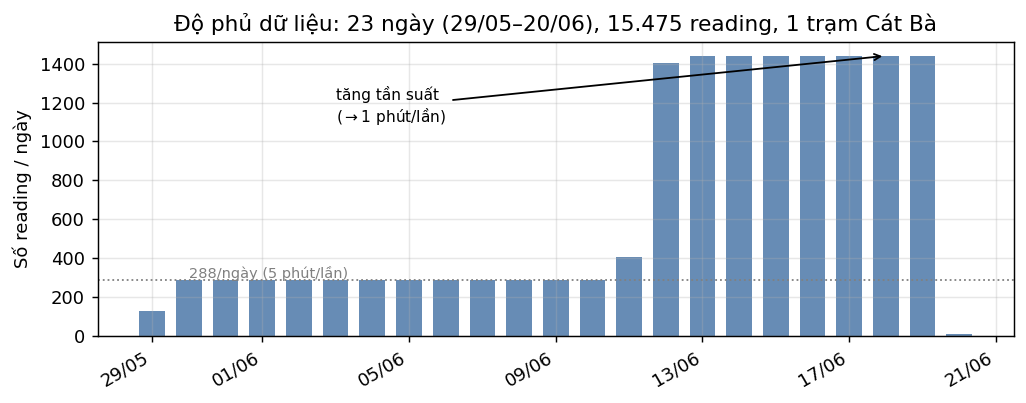
\includegraphics[width=0.92\linewidth]{../figures/data_coverage.png}
\caption{Số reading mỗi ngày. Bước nhảy 12/06 phản ánh thay đổi cấu hình tần suất phía vận hành, không phải sự kiện môi trường.}
\label{fig:coverage}
\end{figure}

\textbf{Thống kê mô tả} (Bảng~\ref{tab:desc}) đã hé lộ bất thường ngay từ trung vị: COD trung vị $=558{,}8$ trùng đúng giá trị lớn nhất (dấu hiệu kẹt trần), NH4 thô hàng trăm lần ngưỡng QCVN.

\begin{table}[h]
\centering\small
\caption{Thống kê mô tả 5 cảm biến (15.475 reading).}
\label{tab:desc}
\begin{tabular}{lrrrrr}
\toprule
\textbf{Chỉ số} & \textbf{min} & \textbf{trung vị} & \textbf{max} & \textbf{độ lệch chuẩn} & \textbf{ngưỡng QCVN B1} \\
\midrule
COD (mg/L)  & 6{,}4  & \textbf{558{,}8} & 558{,}8 & 204{,}0 & 10 \\
NH4 (thô)   & 77{,}6 & 114{,}6 & 160{,}3 & 16{,}7  & --- (xem NH3) \\
pH          & 7{,}78 & 7{,}98  & 8{,}41  & 0{,}10  & 6{,}5--8{,}5 \\
Temp (°C)   & 26{,}6 & 30{,}2  & 33{,}0  & 0{,}76  & --- \\
TSS (mg/L)  & 1{,}1  & 47{,}1  & 237{,}9 & 24{,}0  & 50 \\
\bottomrule
\end{tabular}
\end{table}

\textbf{Phân phối giá trị} (Hình~\ref{fig:dist}) làm rõ hình dạng: COD \emph{lưỡng đỉnh} --- một cụm nhỏ quanh 10 (giai đoạn đầu) và một khối lớn dồn ở trần 558{,}8; pH/Temp tập trung chặt trong dải hợp lý; TSS lệch phải mạnh (42\% reading vượt 50). Diễn biến theo thời gian của bốn cảm biến còn sống ở Hình~\ref{fig:panel}.

\begin{figure}[h]
\centering
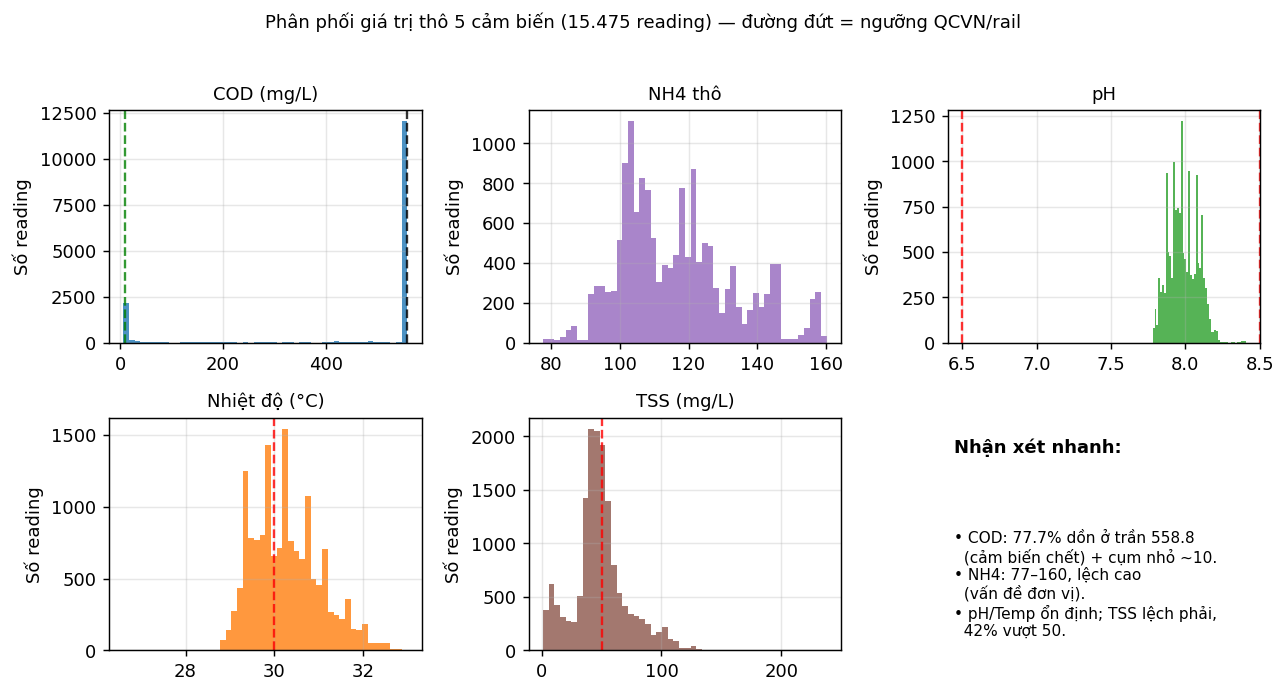
\includegraphics[width=\linewidth]{../figures/value_dist.png}
\caption{Histogram giá trị thô 5 cảm biến. COD dồn ở trần 558{,}8 (cảm biến chết); NH4 lệch cao bất thường; pH/Temp ổn định; TSS lệch phải.}
\label{fig:dist}
\end{figure}

\begin{figure}[h]
\centering
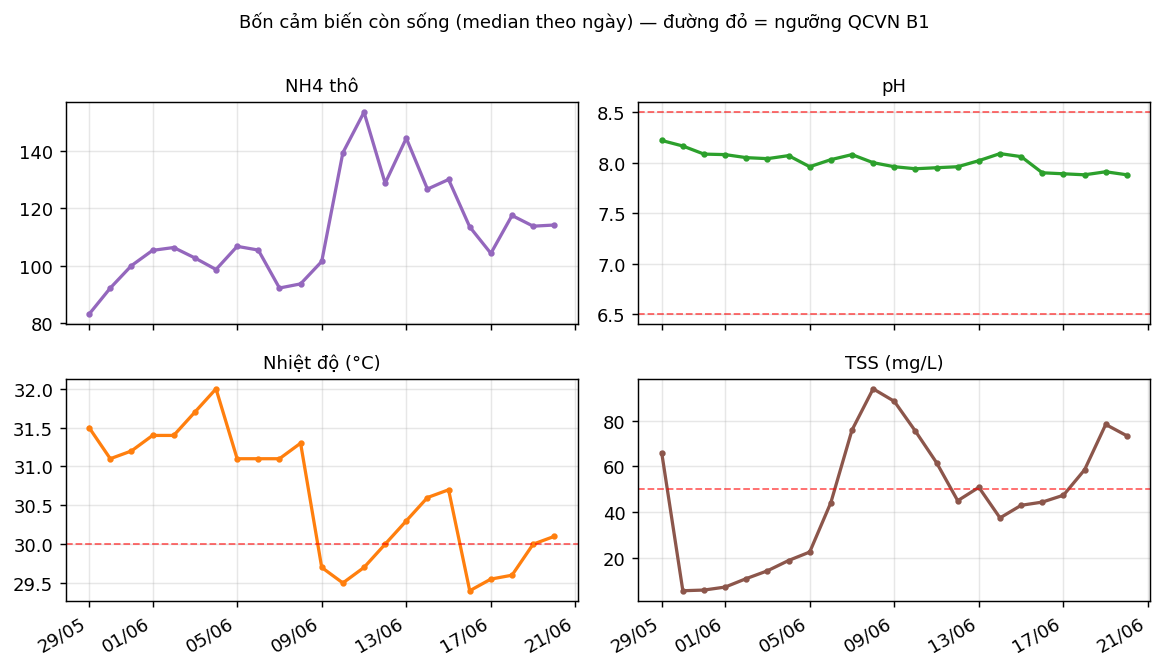
\includegraphics[width=\linewidth]{../figures/sensor_panel.png}
\caption{Diễn biến median theo ngày của bốn cảm biến còn hoạt động. pH, nhiệt độ, TSS dao động hợp lý; NH4 thô ở mức cao (vấn đề đơn vị).}
\label{fig:panel}
\end{figure}

\subsection{Vấn đề phát hiện trong dữ liệu thu thập}
Phân tích trên bộc lộ ba vấn đề cần xử lý trước khi dùng (chi tiết ở Mục~\ref{sec:phuongphap}):
\begin{enumerate}[nosep]
  \item \textbf{Cảm biến COD đã chết} --- 77{,}7\% reading kẹt cứng ở trần 558{,}8 mg/L (phương sai 0), không phải ô nhiễm thật mà là bão hòa cảm biến.
  \item \textbf{Đơn vị NH4 chưa xác định} --- giá trị thô 77--160; nếu là mg/L thì vô lý cho nước nuôi trồng. Thêm nữa cảm biến đo NH4$^+$ trong khi QCVN đánh giá NH3.
  \item \textbf{TSS và nhiệt độ thường xuyên vượt ngưỡng} --- TSS$>$50: 42\% reading; Temp$>$30: 57\% --- đây là tín hiệu thật, cần phản ánh đúng ở phần giám sát.
\end{enumerate}

\subsection{Vấn đề cốt lõi: thiếu chỉ số}
\label{sec:thieuchiso}
Mô hình phân loại cần \textbf{19 chỉ số} (cá giò Hải Phòng) hoặc \textbf{20 chỉ số} (hàu Quảng Ninh); cảm biến chỉ cấp 5. Để lấp khoảng trống, các chỉ số được \textbf{xử lý theo nhóm} (cascade 4 tầng nguồn gốc, Bảng~\ref{tab:gap}) --- ưu tiên đo thật, rồi hóa học, rồi ML, cuối cùng mới trung vị.

\begin{table}[h]
\centering\small
\caption{Cascade 4 tầng: nguồn gốc các chỉ số đưa vào phân loại (mức tin cậy giảm dần từ trên xuống).}
\label{tab:gap}
\begin{tabular}{lll}
\toprule
\textbf{Tầng (nhóm)} & \textbf{Chỉ số / cách lấy} & \textbf{Độ tin} \\
\midrule
1. Đo trực tiếp & pH, nhiệt độ, TSS (+ COD khi QC đạt) & cao nhất \\
2. Suy ra (hóa học) & NH3 (từ NH4 + pH + Temp qua Emerson) & cao \\
3. Nội suy (ML) & DO, BOD5, Transparency, Alkalinity, PO4 & tùy $R^2$ \\
4. Mặc định (trung vị) & Salinity, kim loại nặng, Coliform, H2S, \dots & thấp nhất \\
\bottomrule
\end{tabular}
\end{table}

DO và độ muối là hai chỉ số quan trọng nhất (trọng số 1 và 2 cho cả hàu lẫn cá giò) nhưng đều không đo được trực tiếp --- đây là gốc rễ của các hạn chế nêu ở Mục~\ref{sec:thaoluan}.

\section{Phương pháp}
\label{sec:phuongphap}

\subsection{Phân tích chất lượng dữ liệu}
Mục~\ref{sec:thieuchiso} đã nêu nhanh ba vấn đề; phần này phân tích sâu hai vấn đề chi phối thiết kế pipeline: cảm biến COD chết và đơn vị NH4.

\subsubsection{Cảm biến COD đã hỏng (bão hòa)}
COD diễn biến từ mức hợp lý $\sim$10 mg/L, trôi tăng dần rồi \emph{dính cứng} ở trần 558{,}8 mg/L (Hình~\ref{fig:cod}, Bảng~\ref{tab:cod}).

\begin{table}[h]
\centering\small
\caption{Diễn biến COD theo ngày (median) --- cảm biến trôi rồi chết.}
\label{tab:cod}
\begin{tabular}{lcc}
\toprule
\textbf{Giai đoạn} & \textbf{COD median (mg/L)} & \textbf{\% bản ghi $=558{,}8$} \\
\midrule
29/05 -- 05/06 & $\sim$10 & 0\% \\
06/06 -- 09/06 & 28 $\to$ 128 $\to$ 330 $\to$ 452 & 0\% \\
10/06 & 551 & 46\% \\
11/06 -- 20/06 & 558{,}8 & \textbf{100\%} \\
\bottomrule
\end{tabular}
\end{table}

\begin{figure}[h]
\centering
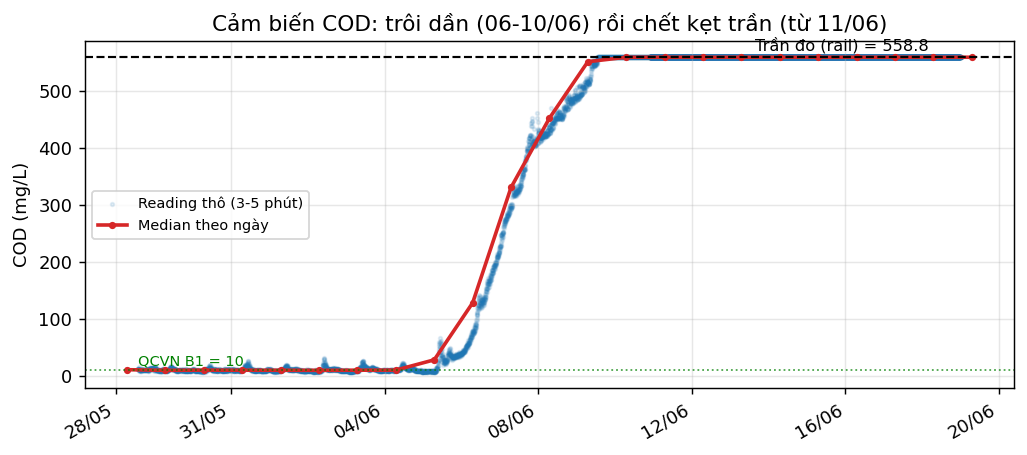
\includegraphics[width=\linewidth]{../figures/cod_timeline.png}
\caption{COD theo thời gian. Phẳng $\sim$10 mg/L tới 05/06, tăng vọt dạng chữ S (06--10/06), rồi kẹt cứng ở trần 558{,}8 --- dấu hiệu rõ của bão hòa cảm biến, không phải ô nhiễm thật.}
\label{fig:cod}
\end{figure}

\warnbox{\textbf{Kết luận:} 558{,}8 lặp lại y hệt trên 12.030 bản ghi liên tiếp (77{,}7\%), phương sai bằng 0 --- đặc trưng \textbf{bão hòa trần đo} (max-range rail), không phải ô nhiễm. Nhiều khả năng do bám bẩn/màng sinh học. Cần báo vận hành vệ sinh, hiệu chuẩn lại đầu dò.}

\subsubsection{Đơn vị NH4 chưa xác định}
NH4 thô dao động 77--160. Nếu là mg/L thì vô lý cho nước nuôi trồng; khả năng cao là $\mu$g/L ($\div 1000 \to 0{,}077$--$0{,}16$ mg/L, sát ngưỡng QCVN 0{,}1) hoặc tín hiệu thô. Ngoài ra cảm biến đo \textbf{NH4$^+$} (ít độc) trong khi QCVN đánh giá theo \textbf{NH3} (rất độc) --- không được ánh xạ thẳng.

\subsection{Kiến trúc 8 module}
\begin{center}\small
\texttt{fetch} $\to$ \texttt{quality} $\to$ \texttt{chemistry} $\to$
\texttt{monitor} $\to$ \texttt{impute} $\to$ \texttt{classify} $\to$ \texttt{report}
\end{center}

\begin{longtable}{ll}
\toprule
\textbf{Module} & \textbf{Trách nhiệm} \\
\midrule \endhead
\texttt{config.py}    & env, registry trạm, ngưỡng QCVN, dải QC, \texttt{NH4\_UNIT\_SCALE} \\
\texttt{chemistry.py} & Quy đổi NH4$^+\to$NH3 (Emerson) \\
\texttt{quality.py}   & QC cảm biến: lọc out-of-range + phát hiện rail/flatline \\
\texttt{fetch.py}     & MongoDB hoặc CSV $\to$ DataFrame; gộp ngày theo median \\
\texttt{monitor.py}   & Kiểm ngưỡng QCVN 10:2023 cột B1 \\
\texttt{impute.py}    & Nội suy thích nghi (dual-model 5/4 feature) + fallback median \\
\texttt{classify.py}  & Ghép đủ chỉ số $\to$ gọi \texttt{src.classification} \\
\texttt{report.py}    & CLI: in giám sát + phân loại + xuất xứ chỉ số \\
\bottomrule
\end{longtable}

\subsection{Quy đổi NH4 $\to$ NH3 (Emerson, 1975)}
\begin{equation}
f = \frac{1}{1 + 10^{(pK_a - pH)}}, \quad
pK_a = 0{,}09018 + \frac{2729{,}92}{T(\text{K})}, \quad
\text{NH3} = \text{NH4}_{\text{raw}} \cdot s \cdot f
\end{equation}
với $s$ là hệ số đơn vị (\texttt{NH4\_UNIT\_SCALE}, mặc định $0{,}001$). Ví dụ NH4$_{\text{raw}}=114{,}59$, pH$=7{,}95$, $T=30^\circ$C: $f\approx0{,}067 \Rightarrow$ NH3 $\approx 0{,}0077$ mg/L.

\warnbox{Đơn vị quyết định kết luận: $s=0{,}001$ cho NH3$=0{,}0077$ (\textbf{đạt}); $s=1{,}0$ cho NH3$=7{,}66$ (\textbf{vượt 76 lần}). Vì vậy đơn vị được tham số hóa và báo cáo luôn in rõ giả định.}

\subsection{Kiểm soát chất lượng (QC)}
Trước khi nội suy, QC chạy hai mức:
\begin{itemize}[nosep]
  \item \textbf{Lọc dòng} ngoài dải vật lý hợp lý (vd COD $\in(0,100)$ $\Rightarrow$ loại bỏ mọi reading $=558{,}8$).
  \item \textbf{Đánh giá chuỗi ngày}: chuỗi phẳng/kẹt trần (flatline, rail-stuck, $CV<10^{-3}$) $\to$ gắn nhãn \texttt{INVALID}.
\end{itemize}
Kết quả QC quyết định \emph{luồng xử lý} ở bước nội suy sau.

\subsection{Mô hình nội suy (XGBoost + LOO-CV theo trạm)}
\label{sec:model}
Ý tưởng: học từ \emph{dữ liệu quan trắc thật} mối quan hệ giữa các chỉ số mà sensor đo được và các chỉ số còn thiếu, rồi áp lên dữ liệu sensor realtime (Hình~\ref{fig:method}).

\begin{figure}[h]
\centering
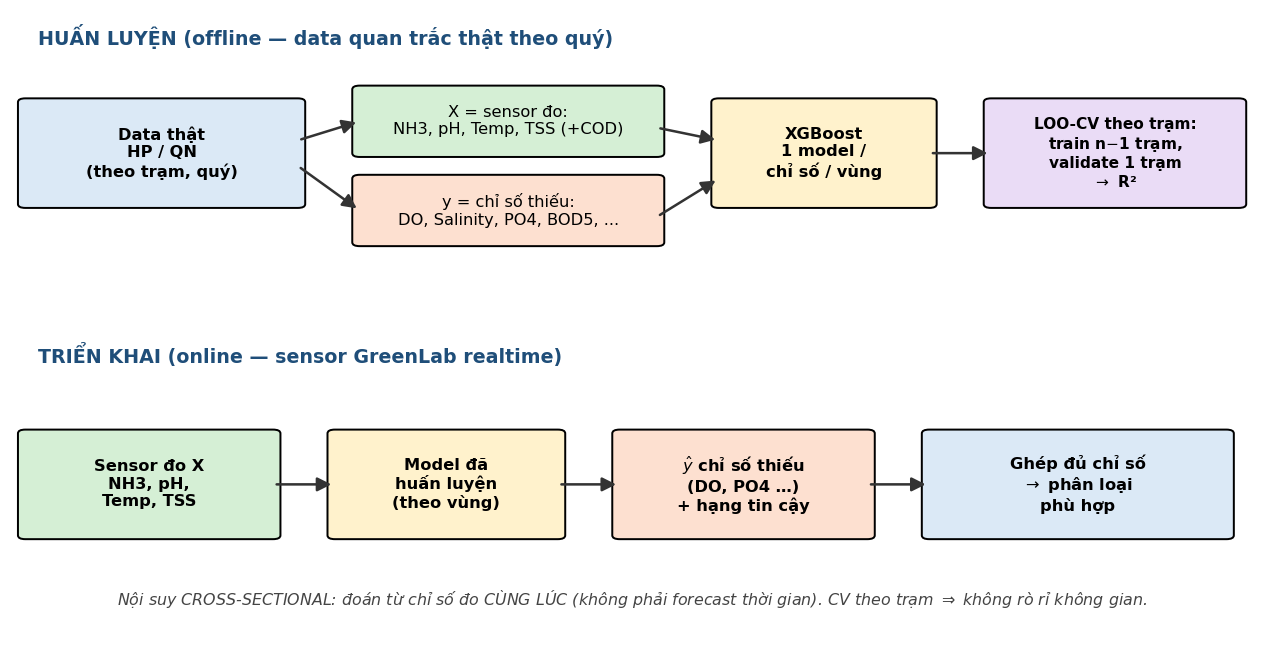
\includegraphics[width=\linewidth]{../figures/impute_method.png}
\caption{Phương pháp nội suy. \textbf{Huấn luyện} (offline): từ data quý HP/QN, đầu vào $X$ = chỉ số sensor đo được, đầu ra $y$ = chỉ số thiếu; mỗi chỉ số một XGBoost; kiểm định LOO-CV theo trạm. \textbf{Triển khai} (online): sensor đo $X$ $\to$ model $\to$ $\hat{y}$ $\to$ phân loại.}
\label{fig:method}
\end{figure}

\begin{itemize}[nosep]
  \item \textbf{Đầu vào} $X$ = chỉ số sensor có: \texttt{[NH3, pH, Temperature, TSS]} ($+$ \texttt{COD} khi sống). Mô phỏng đúng bộ chỉ số GreenLab cấp.
  \item \textbf{Đầu ra} $y$ = chỉ số thiếu cần đoán: DO, \textbf{Salinity}, PO4, BOD5, Transparency, Alkalinity. \emph{Một} mô hình cho \emph{mỗi} chỉ số $\times$ \emph{mỗi} vùng.
  \item \textbf{Kiểm định} = \textbf{Leave-One-Station-Out CV}: huấn luyện trên $n-1$ trạm, dự đoán trạm bị giữ lại, lặp cho mọi trạm rồi gộp $\to R^2$. Chia theo \emph{trạm} (không theo thời gian) để tránh rò rỉ không gian.
\end{itemize}

\warnbox{Đây là nội suy \textbf{cross-sectional} --- đoán giá trị một chỉ số từ các chỉ số đo \emph{cùng thời điểm}, \emph{không phải} dự báo (forecast) theo thời gian. Vì vậy chỉ cần một bản ghi sensor là suy ra được, không cần chuỗi lịch sử.}

\subsubsection{Thuật toán: XGBoost (gradient boosting trees)}
Mỗi mô hình nội suy là một \textbf{XGBoost} (\texttt{XGBRegressor}) --- gradient boosting trên cây quyết định. Lý do chọn:
\begin{itemize}[nosep]
  \item \textbf{Phù hợp dữ liệu bảng}, ít mẫu (HP chỉ 216 dòng): cây boosting học tốt quan hệ phi tuyến mà không cần chuẩn hóa đặc trưng, ít nhạy outlier hơn mô hình tuyến tính.
  \item \textbf{Tương quan phi tuyến} giữa chỉ số sinh-hóa (vd Salinity vs NH3/TSS theo gradient cửa sông) — cây nắm được, hồi quy tuyến tính thì không.
  \item \textbf{Nhất quán với hệ thống chính} của đồ án (XGBoost đã là phương pháp lõi cho dự báo + phân loại), dễ tái dùng hạ tầng.
\end{itemize}

\begin{table}[h]
\centering\small
\caption{Siêu tham số XGBoost (đồng nhất mọi chỉ số/vùng).}
\label{tab:xgb}
\begin{tabular}{ll}
\toprule
\textbf{Tham số} & \textbf{Giá trị} \\
\midrule
\texttt{n\_estimators} & 100 (số cây) \\
\texttt{max\_depth}    & 4 (giữ cây nông, chống overfit data nhỏ) \\
\texttt{learning\_rate}& 0{,}1 \\
\texttt{random\_state} & 42 (tái lập) \\
objective & \texttt{reg:squarederror} (hồi quy) \\
\bottomrule
\end{tabular}
\end{table}

Số cây vừa phải $+$ cây nông là lựa chọn có chủ đích cho tập huấn luyện nhỏ: đủ học quan hệ chính nhưng tránh khớp quá. Kết quả LOO-CV (Mục~\ref{sec:r2}) cho thấy mô hình \emph{không} tự khớp ảo --- phần lớn chỉ số R² thấp/âm đúng như kỳ vọng khi không có tín hiệu.

\subsection{Hai luồng xử lý của bước nội suy}
\label{sec:hailuong}
Phần suy ra chỉ số thiếu được tổ chức theo \textbf{hai trục quyết định độc lập}. Trục nào cũng do dữ liệu thực ép ra, không phải lựa chọn tùy ý.

\subsubsection{Luồng 1 --- thích nghi theo trạng thái COD (5-feature vs 4-feature)}
Vì cảm biến COD chết phần lớn thời gian, mô hình nội suy phải \emph{thích nghi} theo kết quả QC của COD:
\begin{itemize}[nosep]
  \item \textbf{COD VALID} (giai đoạn đầu, $<6$\% reading): dùng bộ \textbf{5-feature} [COD, NH3, pH, Temp, TSS]. Các dòng COD lỗi đã bị QC \emph{cắt bỏ} khỏi tập huấn luyện/suy luận.
  \item \textbf{COD INVALID} (đa số): rớt COD, dùng bộ \textbf{4-feature} [NH3, pH, Temp, TSS]. Không bịa COD bằng median (sẽ kéo lệch toàn bộ).
\end{itemize}
Hai bộ được huấn luyện sẵn; QC chọn bộ tại thời điểm chạy. Ngày 20/06 (COD chết) $\to$ tự động dùng 4-feature.

\subsubsection{Luồng 2 --- huấn luyện theo vùng (HP-only vs HP+QN gộp)}
Mô hình nội suy được train trên \emph{dữ liệu quan trắc thật} theo quý. Câu hỏi: trạm Cát Bà (HP) nên học từ data nào?
\begin{itemize}[nosep]
  \item \textbf{HP-only} (216 dòng, 14 trạm Hải Phòng) --- cùng vùng với trạm đích.
  \item \textbf{HP+QN gộp} (thêm 1.552 dòng, 97 trạm Quảng Ninh) --- nhiều mẫu hơn nhưng khác chế độ thủy văn.
\end{itemize}
Hai vịnh khác chế độ làm quan hệ sensor$\to$DO mâu thuẫn khi gộp; kết quả (Mục~\ref{sec:r2}) cho thấy tách HP-only \emph{cứu} được dự đoán DO mà gộp đã phá. Vì vậy chọn huấn luyện \textbf{riêng theo vùng}.

\subsubsection{Kết hợp hai luồng}
Bảng~\ref{tab:hailuong} là ma trận $2\times2$. Mỗi ô là một bộ mô hình riêng; thực thi chọn ô theo (vùng trạm $\times$ trạng thái COD).

\begin{table}[h]
\centering\small
\caption{Ma trận hai luồng. Trạm Cát Bà 20/06 rơi vào ô \textbf{HP-only $\times$ 4-feature}.}
\label{tab:hailuong}
\begin{tabular}{lcc}
\toprule
& \textbf{COD VALID (5-feat)} & \textbf{COD INVALID (4-feat)} \\
\midrule
\textbf{HP-only}     & 5 cột$^*$ & 4 cột \textbf{(Cát Bà 20/06)} \\
\textbf{HP+QN gộp}   & 5 cột & 4 cột \\
\bottomrule
\end{tabular}

{\footnotesize $^*$ Data HP không có cột COD/BOD5/Alkalinity nên ``5-feature'' ở HP thực chất chỉ 4 cột; code lưu đúng danh sách cột mỗi vùng (\texttt{feat\_cols.json}) để vector suy luận không lệch.}
\end{table}

Sau khi nội suy, kiểm định \textbf{LOO-CV theo trạm} và phân hạng theo \textbf{chính sách 3 mức tin cậy} (chi tiết Mục~\ref{sec:r2}): $R^2\ge0{,}4$ dùng model (ML-mạnh); $0{,}2\le R^2<0{,}4$ vẫn dùng nhưng gắn cờ độ tin thấp (ML-yếu); $R^2<0{,}2$ thay bằng trung vị vùng. Hai chỉ số artifact (BOD5, Alkalinity) bị loại bất kể $R^2$. Cuối cùng ghép \texttt{measured} $\oplus$ \texttt{imputed} $\oplus$ \texttt{defaulted} $\to$ chấm điểm piecewise-linear theo breakpoint chuyên gia (\texttt{src.classification}).

\section{Kết quả thực nghiệm}

\subsection{Kết quả nội suy từng chỉ số (LOO-CV $R^2$)}
\label{sec:r2}
Sáu chỉ số nội suy được kiểm định chéo Leave-One-Station-Out trên cả hai vùng và hai bộ feature. Hình~\ref{fig:r2all} trực quan toàn bộ; phân hạng theo chính sách 3 mức bên dưới.

\begin{figure}[h]
\centering
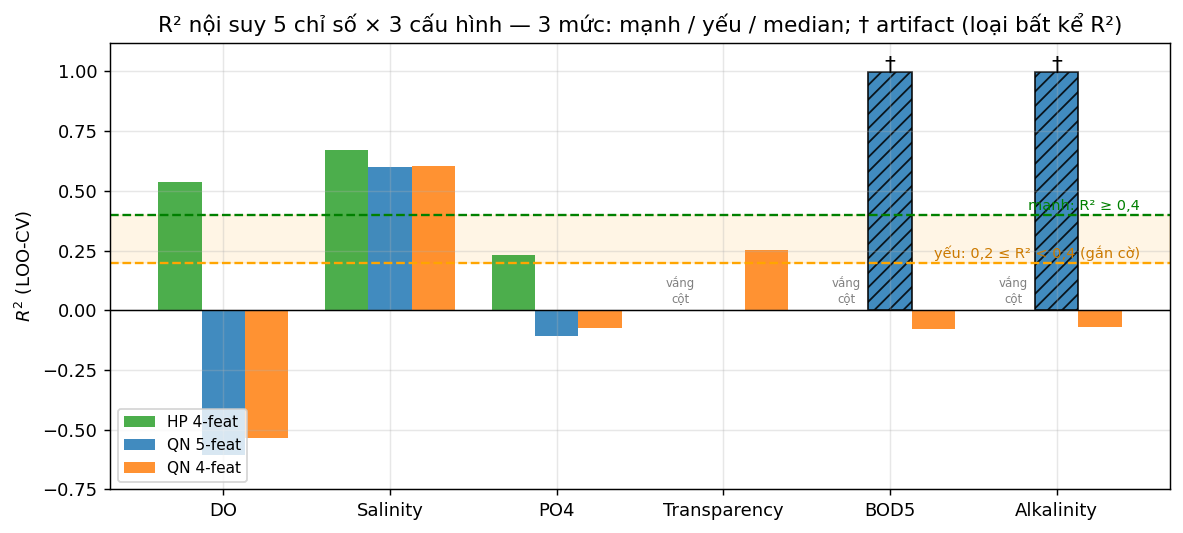
\includegraphics[width=\linewidth]{../figures/r2_all.png}
\caption{$R^2$ của 6 chỉ số $\times$ 3 cấu hình. \textbf{DO (HP)} và \textbf{Salinity (cả 2 vùng)} vượt ngưỡng $0{,}4$ một cách \emph{thực}. Hai cột gạch chéo ($\dagger$ BOD5/Alkalinity ở QN 5-feat) chạm $\approx1{,}0$ nhưng là artifact (Mục~\ref{sec:thaoluan}). Cột ``vắng cột'' = chỉ số đó không có trong dữ liệu HP.}
\label{fig:r2all}
\end{figure}

\textbf{Chính sách 3 mức tin cậy.} Thay vì một ngưỡng cứng, chỉ số được phân hạng theo $R^2$:
\begin{itemize}[nosep]
  \item \textbf{ML-mạnh} ($R^2\ge0{,}4$): dùng model, tin.
  \item \textbf{ML-yếu} ($0{,}2\le R^2<0{,}4$): dùng model \emph{nhưng gắn cờ ``độ tin thấp''} ở xuất xứ.
  \item \textbf{Median} ($R^2<0{,}2$): trung vị vùng.
  \item \textbf{Artifact} (BOD5, Alkalinity): loại \emph{bất kể} $R^2$ (xem dưới).
\end{itemize}

\begin{table}[h]
\centering\small
\caption{$R^2$ kiểm định chéo + hạng tin cậy mỗi chỉ số. HP 5-feat = 4-feat (HP không có cột COD).}
\label{tab:r2}
\begin{tabular}{lcccl}
\toprule
\textbf{Chỉ số} & \textbf{HP (4-feat)} & \textbf{QN 5-feat} & \textbf{QN 4-feat} & \textbf{Hạng / kết quả dùng} \\
\midrule
DO            & \textbf{0{,}535} & $-0{,}606$ & $-0{,}537$ & HP: \textbf{ML-mạnh}; QN: median \\
Salinity      & \textbf{0{,}673} & \textbf{0{,}599} & \textbf{0{,}602} & \textbf{ML-mạnh cả 2 vùng} \\
PO4           & $0{,}233$ & $-0{,}108$ & $-0{,}074$ & HP: \textbf{ML-yếu} (cờ); QN: median \\
Transparency  & --- & $-0{,}003$ & $0{,}254$ & QN: \textbf{ML-yếu} (cờ); HP: vắng cột \\
BOD5          & --- & $0{,}9999^\dagger$ & $-0{,}078$ & \textbf{artifact} $\to$ median \\
Alkalinity    & --- & $0{,}9995^\dagger$ & $-0{,}072$ & \textbf{artifact} $\to$ median \\
\bottomrule
\end{tabular}

{\footnotesize ``---'' = data HP không có cột. $^\dagger$ artifact COD-driven, loại bất kể $R^2$ (Mục~\ref{sec:thaoluan}).}
\end{table}

\textbf{Đọc theo từng chỉ số:}
\begin{itemize}[nosep]
  \item \textbf{DO} --- chỉ số quan trọng nhất. HP-only $R^2=0{,}535$ (ML-mạnh); QN $<0$ (median).
  \item \textbf{Salinity} --- chỉ số quan trọng \emph{thứ hai} (importance\_rank 4), \textbf{đoán được mạnh ở CẢ hai vùng} ($0{,}673$ HP, $0{,}60$ QN). Hợp lý vật lý: gradient cửa sông (nước ngọt vào $\to$ độ muối $\downarrow$, dinh dưỡng/đục $\uparrow$). Ban đầu để median do giả định sai; data đính chính.
  \item \textbf{PO4} --- HP $0{,}233$ rơi vào \textbf{ML-yếu}: dùng nhưng gắn cờ độ tin thấp (chỉ tốt hơn median $\sim$12\% RMSE). QN âm.
  \item \textbf{Transparency} --- HP không có cột; QN 4-feat $0{,}254$ là \textbf{ML-yếu} (dùng cho trạm QN, có cờ).
  \item \textbf{BOD5, Alkalinity} --- QN 5-feat $\approx1{,}0$ nhưng \textbf{artifact}: tương quan tất định với COD (Mục~\ref{sec:thaoluan}); bỏ COD thì $R^2$ rớt âm. \emph{Loại bất kể} $R^2$ cao.
\end{itemize}

\warnbox{\textbf{Tổng kết nội suy (chính sách 3 mức):} \textbf{2 mạnh} (DO ở HP, Salinity ở cả 2 vùng) $+$ \textbf{2 yếu có cờ} (PO4 ở HP, Transparency ở QN); BOD5/Alkalinity loại do artifact. Riêng trạm \textbf{Cát Bà} (HP, 4-feat): DO (mạnh) $+$ Salinity (mạnh) $+$ PO4 (yếu) $= 3$ chỉ số ML-grounded, phần còn lại median. Đặc biệt Salinity --- chỉ số quan trọng thứ 2 --- chuyển từ hằng số sang model-grounded, vá một phần hạn chế H2.}

\textbf{Phát hiện then chốt (Luồng 2):} tách \textbf{HP-only} \emph{cứu} được DO từ $R^2<0$ (gộp QN+HP) lên $R^2=0{,}535$ (Hình~\ref{fig:do}). \textbf{Luồng 1:} DO ở HP đoán được \emph{ngang nhau} ở cả 5-feature lẫn 4-feature (cùng $0{,}535$, vì HP vốn không có cột COD), nên trạm Cát Bà vẫn có DO \emph{model-grounded} kể cả khi COD chết --- đúng ô \textbf{HP-only $\times$ 4-feat} (Bảng~\ref{tab:hailuong}).

\begin{figure}[h]
\centering
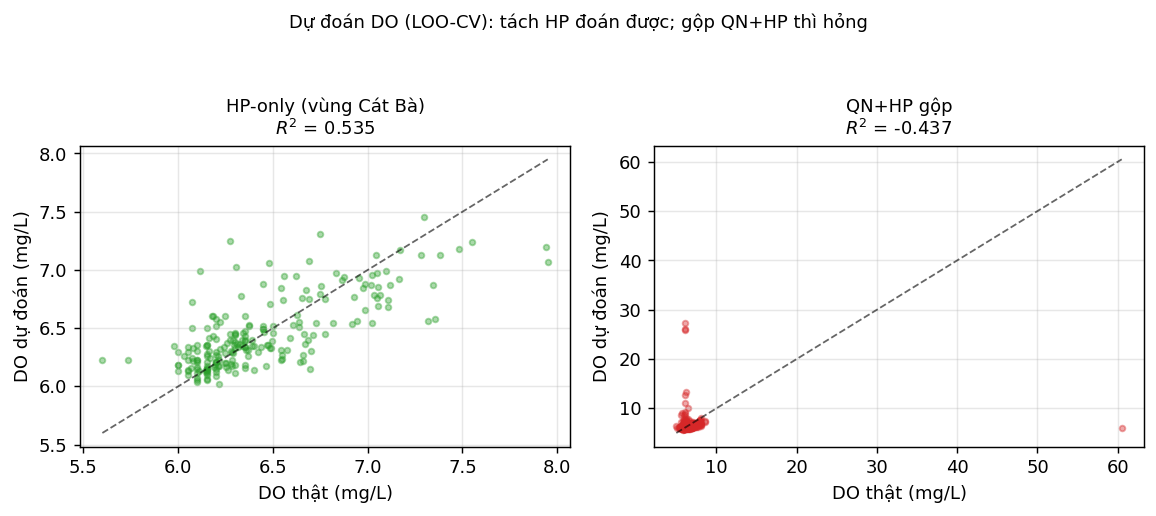
\includegraphics[width=\linewidth]{../figures/do_per_region.png}
\caption{Dự đoán DO (LOO-CV). HP-only: điểm bám đường chéo, $R^2=0{,}535$. Gộp QN+HP: phân tán, $R^2<0$ (tệ hơn trung vị). Tách vùng là yếu tố quyết định.}
\label{fig:do}
\end{figure}

\subsection{Vì sao các chỉ số còn lại để median --- bằng chứng}
\label{sec:median-evidence}
Quyết định để các chỉ số còn lại (kim loại nặng, Coliform, H2S, COD) dùng trung vị \emph{không} phải võ đoán --- chúng tôi đã chạy LOO-CV cho \emph{tất cả} (Hình~\ref{fig:medr2}). Kết quả:
\begin{itemize}[nosep]
  \item \textbf{Salinity là ngoại lệ duy nhất} đoán được ổn định cả 2 vùng ($R^2\approx0{,}6$) $\Rightarrow$ đã chuyển sang ML-target.
  \item \textbf{Kim loại QN} (As, Cd, Pb, Cu, Hg, Zn, Cr): $R^2$ đều $<0{,}2$ (phần lớn âm) --- không có tín hiệu từ 4 input sensor (kim loại đến từ nguồn thải, không liên quan pH/nhiệt/NH3/TSS).
  \item \textbf{Vài kim loại HP} ($R^2>0{,}2$: Cu, Zn, As) là \emph{nhiễu}: cột gần-LOD (median $\approx0$, phương sai bé) và \textbf{không lặp lại} ở QN (97 trạm) --- không đáng tin.
  \item \textbf{Cd, Pb, Total\_Cr ở HP}: $R^2=1{,}0$ \emph{degenerate} --- cột hằng số (phương sai 0); median đã bằng đúng hằng số đó nên ML vô nghĩa.
  \item \textbf{Coliform, H2S, COD}: $R^2<0$.
\end{itemize}

\begin{figure}[h]
\centering
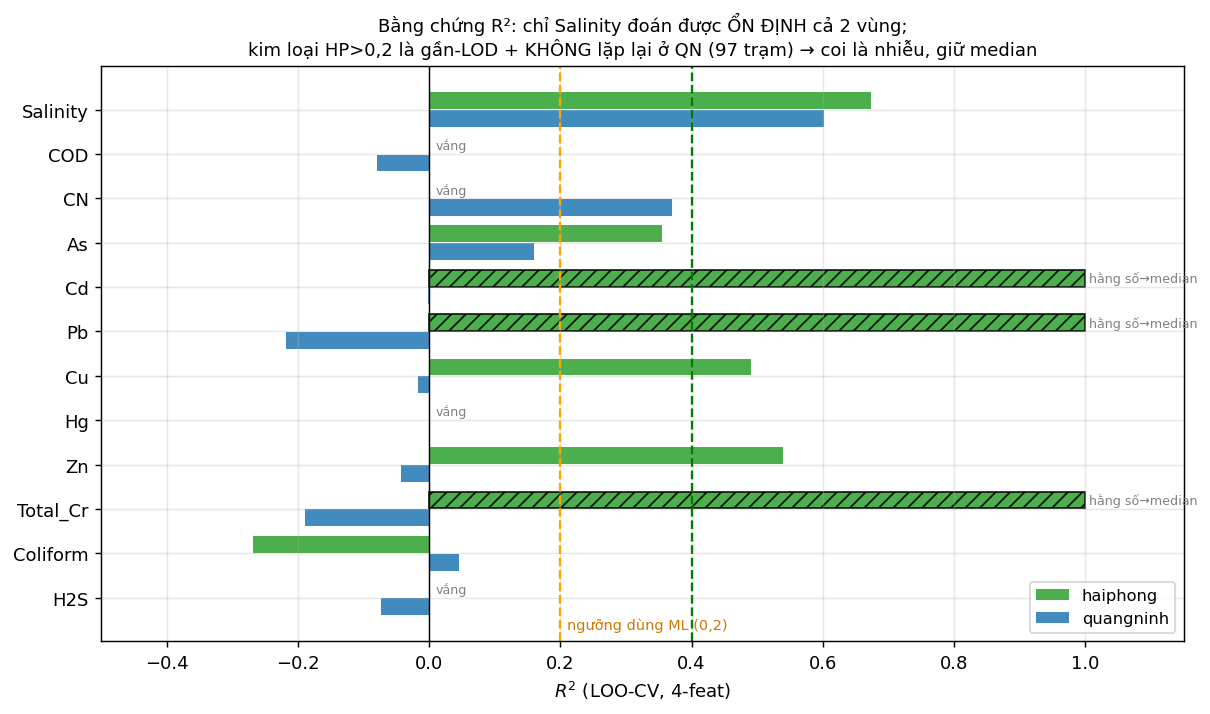
\includegraphics[width=\linewidth]{../figures/median_params_r2.png}
\caption{LOO-CV $R^2$ của các chỉ số median-default. Chỉ Salinity vượt ngưỡng ở cả 2 vùng. Kim loại HP có $R^2>0$ nhưng gần-LOD và không lặp lại ở QN; ba cột gạch chéo là hằng số ($R^2=1{,}0$ degenerate).}
\label{fig:medr2}
\end{figure}

\subsection{Chạy CLI thực tế}
Bộ test: \textbf{37/37 PASS}. Hai ví dụ báo cáo (trạm Cát Bà, vùng HP):

\begin{lstlisting}
# Ngay 2026-06-20 (COD chet -> 4feat, vung haiphong)
COD sensor: INVALID
[MONITORING] NH3 0.0068 (QCVN <=0.1) OK | pH 7.89 (6.5-8.5) OK
             Temp 30.2 EXCEED | TSS 75.8 EXCEED
[CLASSIFICATION - COBIA | vung haiphong] Score 0.900 -> "Phu hop"
  feature_set: 4feat | imputed_fraction: 71%
  ML-manh (R2>=0.4): DO, Salinity | ML-yeu (0.2<=R2<0.4): PO4
  imputed = {DO: 6.20 (manh), Salinity: 30.34 (manh), PO4: 0.042 (yeu)}
  defaulted = {As, Cd, Pb, Cu, ...}   # kim loai/Coliform/H2S -> median

# Ngay 2026-06-01 (COD song -> 5feat)
COD sensor: VALID
[MONITORING] COD 9.8 (QCVN <=10) OK | ...
[CLASSIFICATION - COBIA] Score 0.953 -> "Rat phu hop" | feature_set: 5feat
\end{lstlisting}

Phần giám sát QCVN hoạt động đúng: ngày 20/06 báo Temp và TSS vượt ngưỡng, COD bị QC loại nên không báo EXCEED giả. Phần phân loại tuy chạy nhưng cần đọc kèm các hạn chế ở mục sau.

\section{Thảo luận và kết luận}
\label{sec:thaoluan}

\subsection{Hạn chế (phải nêu rõ)}
Kết quả \emph{chạy được} không đồng nghĩa với \emph{đáng tin}.

\textbf{H1 --- Nội suy đóng góp một phần (chính sách 3 mức).}
Với scope gộp QN+HP ban đầu, đường 4-feature fail hết $\Rightarrow$ 100\% trung vị. Sau khi \textbf{tách HP-only} $+$ áp \textbf{chính sách 3 mức} $+$ bổ sung Salinity, trạm Cát Bà có \textbf{3 chỉ số ML-grounded}: DO (mạnh, $0{,}535$), Salinity (mạnh, $0{,}673$) $+$ PO4 (yếu, $0{,}233$, có cờ). Kim loại, Coliform, H2S vẫn là trung vị --- đã kiểm định không đoán được (Mục~\ref{sec:median-evidence}).

\textbf{H2 --- Nhãn vẫn lệch về ``phù hợp'' (đã giảm nhờ Salinity).}
Ngày 20/06 TSS và nhiệt độ đều vượt ngưỡng, nhưng nhãn vẫn ``phù hợp'' ($0{,}900$), vì $\sim$71\% đầu vào vẫn là trung vị ``nước khỏe'' nuốt chửng các chỉ số thật. Việc đưa \textbf{Salinity} (chỉ số quan trọng thứ 2) từ hằng số sang model-grounded đã \emph{giảm} mức chi phối của hằng số, nhưng kim loại/Coliform vẫn cố định nên nhãn nối đất còn yếu.

\textbf{H3 --- $R^2\approx0{,}9999$ của BOD5/Alkalinity là artifact.}
Tương quan BOD5--COD $=0{,}977$ và Alkalinity--COD $=0{,}955$ (không có cơ sở hóa học). Hình~\ref{fig:artifact} cho thấy các điểm nằm trên một đường gần như \emph{tất định} --- quan hệ hàm do quá trình sinh dữ liệu, không phải tương quan sinh thái học được. ``Thành công'' của 5-feature phụ thuộc hoàn toàn vào COD --- đúng cảm biến đã chết.

\begin{figure}[h]
\centering
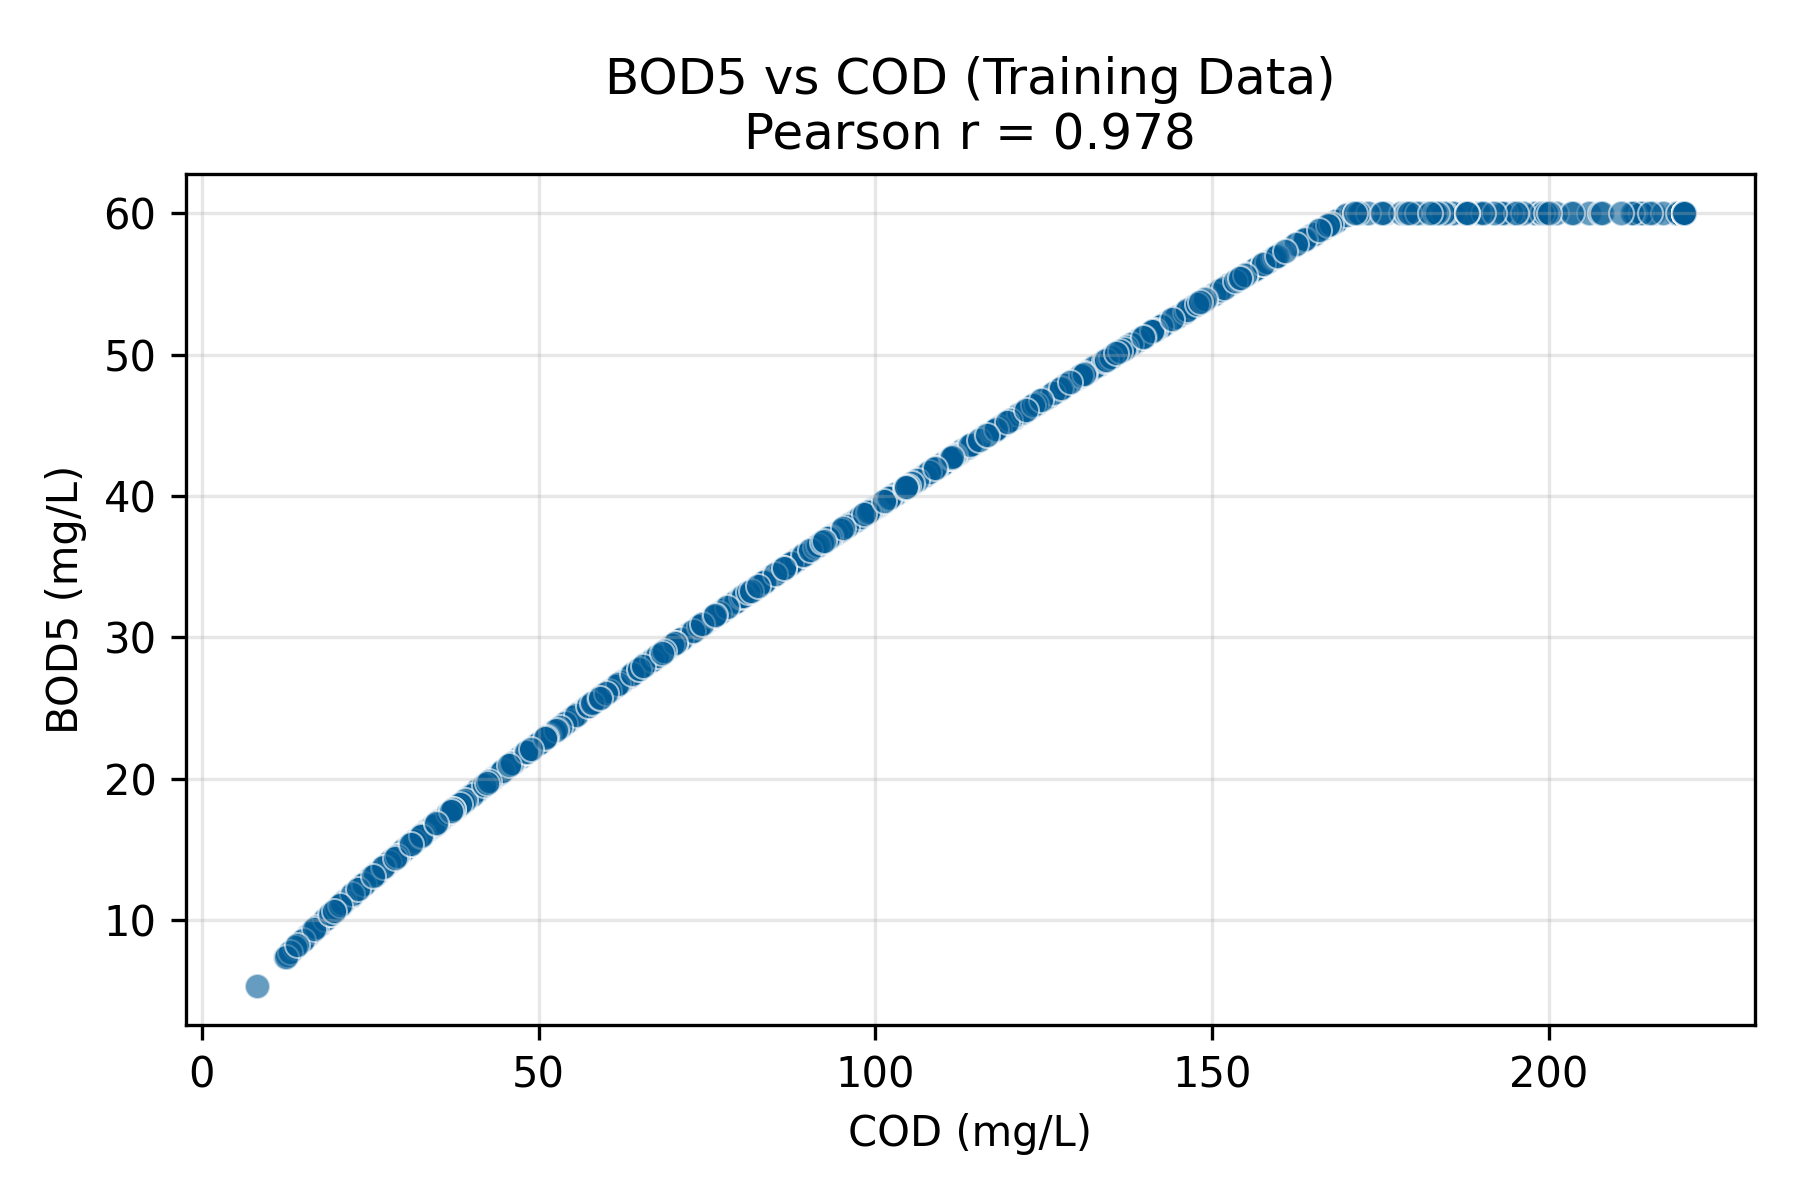
\includegraphics[width=\linewidth]{../figures/bod5_cod_scatter.png}
\caption{BOD5 và Alkalinity trong dữ liệu huấn luyện QN/HP gần như là hàm tất định của COD (điểm bám sát một đường). Đây là lý do $R^2$ chạm 0{,}999 --- artifact của dữ liệu, không phải khả năng dự báo thực.}
\label{fig:artifact}
\end{figure}

\textbf{H4 (đã đính chính) --- DO dự báo được KHI tách đúng vùng.}
Kết luận trước (``DO không đoán được'') là \emph{artifact của scope gộp QN+HP}: trộn hai vịnh khác chế độ làm nhiễu quan hệ. Tách HP-only $\Rightarrow$ DO đạt $R^2=0{,}535$ (Hình~\ref{fig:do}) --- mức vừa nhưng hơn hẳn trung vị. Bài học phương pháp: \emph{chọn sai phạm vi dữ liệu có thể che giấu tín hiệu thật}. Riêng QN, DO vẫn không đoán được ($R^2<0$) --- cần xem lại khi bật trạm Vân Đồn.

\warnbox{\textbf{Khuyến nghị sử dụng:} phần \emph{giám sát QCVN} (5 chỉ số thật) hữu ích và đáng tin. Phần \emph{phân loại} hiện chỉ nên trình bày như \textbf{pipeline demo}, chưa đủ tin cậy để ra quyết định nuôi trồng cho tới khi: (a) bổ sung cảm biến DO + độ muối, (b) sửa cảm biến COD, (c) xác nhận đơn vị NH4.}

\subsection{Kết luận và hướng phát triển}
Module \texttt{lab/realtime\_greenlab/} đã thiết lập đầy đủ đường ống từ MongoDB thời gian thực tới nhãn phù hợp, kèm kiểm soát chất lượng cảm biến, quy đổi hóa học NH3, và nội suy thích nghi theo vùng --- toàn bộ kèm cảnh báo xuất xứ minh bạch. Quá trình cho thấy hai bài học phương pháp: (1) \emph{kiểm tra dữ liệu trước khi tin mô hình} (phát hiện COD chết); (2) \emph{phạm vi dữ liệu huấn luyện quyết định kết quả} (tách HP-only cứu tín hiệu DO mà scope gộp đã che giấu). Đây là kết quả khoa học trung thực, đáng nêu trong luận văn hơn một con số ``phù hợp'' đẹp nhưng rỗng.

\textbf{Hướng phát triển:}
\begin{enumerate}[nosep]
  \item Kích hoạt thu thập trạm Vân Đồn (QN) để mở rộng sang oyster.
  \item Bổ sung cảm biến DO + độ muối --- hai chỉ số hiện đang là hằng số.
  \item Xác nhận đơn vị NH4 với nhà cung cấp; cập nhật \texttt{NH4\_UNIT\_SCALE}.
  \item Khi đủ chuỗi thời gian, thử dự báo (forecast) chỉ số tương lai thay vì chỉ phân loại tức thời.
  \item Tích hợp phần giám sát QCVN (đã đáng tin) vào webapp.
\end{enumerate}


\end{document}
